\documentclass{llncs}
% \documentclass[twocolumn]{article}

% \usepackage{latexsym}
% \usepackage{amssymb}
\usepackage{graphicx}
% \usepackage{cite}
\usepackage{url}
% \usepackage{soul}
% \usepackage{multirow}
% \usepackage{listings}
% \setstcolor{red}
% \usepackage[utf8]{inputenc}
% \usepackage[T1]{fontenc}

% \usepackage{comment}
% \usepackage{times}

%%%%%%%%%%%%%%%%%%%%%%%%%%%%%%%%%%%%%%%%%%%%%%%%%%%%%%%%%%%%%%%%%%%%%%%

\newcommand{\hcinv}{\texttt{hc\_inversion}\xspace}
\newcommand{\coqdockw}[1]{\texttt{#1}}
\newcommand{\inversion}{\coqdockw{inversion}\xspace}
\newcommand{\inv}{\coqdockw{inv}\xspace}
\newcommand{\simlight}{\texttt{Simlight}\xspace}
\newcommand{\compcert}{\texttt{CompCert}\xspace}
\newcommand{\clight}{\texttt{Clight}\xspace}
\newcommand{\simsoc}{\texttt{SimSoC}\xspace}
\newcommand{\simsoccert}{\texttt{SimSoC-Cert}\xspace}
\newcommand{\stt}{\small\tt}
\newcommand{\why}{\texttt{Why}\xspace}
\newcommand{\whyML}{\texttt{WhyML}\xspace}
\newcommand{\whyCert}{\texttt{WhyCert}\xspace}
\newcommand{\framac}{\texttt{Frama-C}\xspace}


%replace XXX with the submission number you are given from the ASPLOS submission site.
\newcommand{\asplossubmissionnumber}{28}
\usepackage[normalem]{ulem}
\usepackage{xspace}
\usepackage{alltt}
\usepackage{amsmath}
\usepackage{extarrows}

\pagestyle{plain}
\begin{document}
%date not printed
\date{}

\title{Towards Verified Faithful Simulation}
%\author{Authors omitted for review\\room for authors addresses\\}
\author{%
Vania Joloboff\inst{1}
\and Jean-Fran\c{c}ois Monin\inst{2}
\and Xiaomu Shi\inst{3}
}
\institute{%
East China Normal University - INRIA - LIAMA
\and Universit\'{e} de Grenoble - Verimag
\and Tsinghua University
}
\authorrunning{V. Joloboff, J.-F. Monin \& X. Shi}
\maketitle
\thispagestyle{empty}

\begin{abstract}
  This paper presents an approach to construct a verified virtual
  prototyping framework of embedded software. The machine code
  executed on a simulated target architecture can be proven to provide
  the same results as the real hardware, and the proof is verified
  with a theorem prover. The method consists in proving each
  instruction of the instruction set independently, by proving that
  the execution of the C code simulating an instruction yields an
  identical result to that obtained by a formal executable model of
  the processor architecture. This formal model itself is obtained
  through an automated translation process from the architecture
  specifications. Each independent proof draws a number of lemmas from
  a generic lemma library and also uses the automation of inversion
  tactics in the theorem prover. The paper presents the proof of the
  ARM architecture version 6 Instruction Set Simulator of the SimSoC
  open source simulator, with all of the proofs being verified by the
  Coq proof assistant, using automated tactics to reduce manual proof
  development.
\end{abstract}
\section{Introduction}

In many embedded systems applications nowadays, virtual prototyping is
used to design, develop and test new applications. Most of these
virtual prototypes include an Instruction Set Simulator (ISS) to
simulate the target processor. The ISS runs the target executable
binary code in emulating the hardware and generate the outputs that
the executable should produce when run on the target platform. An ISS
can be used for example to optimize algorithms such as cryptographic
software, or to debug new compiler developments, or in the design of
many embedded systems applications.  Instead of using real hardware
prototypes, simulated platforms are more convenient and less
expensive.  Then, it is important to be sure that the simulator
used is faithful to the hardware that it emulates.  A {\em faithful
  ISS} must produce exactly the same results as the executable would
if run on hardware implementation of the instruction set
specification, and this guarantee must be proven.

The purpose of our work is to formally verify that the execution of a
program on our Instruction Set Simulator for the target ARM
architecture indeed produces the expected results, to be certain that
the data output from the simulator, the final processor and memory
states are indeed identical to the result obtained with the real
hardware. This requires sequential steps, to prove first that the
translation from the C code of the simulator to the simulation machine
is correct, and second that the simulation of the target machine code
is also correct, that is, it preserves the semantics of the computer
architecture, together with the fact that all of these proofs are
verified using a theorem prover, or proof checker, not subject to human
error in the proof elaboration or verification.

The next sections of the paper are organized as follows. Section 2
reviews related work. Section 3 describes the tools that we have used,
in particular the Compcert~C compiler, a certified compiler for the C
language, the Coq proof assistant, and the \simsoc simulator in which
our work is integrated.  Section 4 presents our contribution to prove
the correctness of an ARM Instruction Set Simulator, integrated within
SimSoC. In summary, the method consists in proving each instruction of
the instruction set independently, by proving that the execution of
the C code simulating an instruction yields identical result to that
obtained by a formal executable model of the architecture.
% This formal model itself is obtained with automated translation process from the
%architecture specifications.
Each independent proof requires using a number of lemmas from a
generic lemmas library and usage of a new inversion tactics in the
theorem prover.  Finally, our conclusion mentions lessons learned and
directions for future work.

%%%%%%%%%%%%%%%%%%%%%%%%%%%%%%%%%%%%%%%%%%%%%%%%%%%%%%%%%%%%%%%%%%%%%%%%%%%%%
\section{Related Work}
\label{related}

Program certification has to be based on a formal model of the program
under study.  Such a formal model is itself derived from a formal
semantics of the programming language.
Axiomatic semantics and Hoare logic %\cite{Floyd67,Hoare-1969}
have been widely used for proving the correctness of programs.  For
imperative programming languages such as C, a possible approach is to
consider tools based on axiomatic semantics, like
\framac~\cite{canet2009value}, a framework for a set of interoperable
program analyzers for C. Most of the modules integrated inside rely on
ACSL (ANSI/ISO C Specification Language), a specification language
based on an axiomatic semantics for C.
% ACSL is powerful enough to
%express axiomatizations directly at the level of the C program.  State
%labels can be defined to denote a program control point, and can then
% be used in logic functions and predicates.

\framac software leverages off from \why technology
\cite{bobot2011why3,filliatre07cav}, a platform for deductive program
verification, which is an implementation of Dijkstra's calculus of
weakest preconditions.  \why compiles annotated C code into an
intermediate language.  The result is given as input to the VC
(Verification Conditions) generator, which produces formulas to be
sent to both automatic provers or interactive provers like Coq.

%% JF: Not very useful here
% Paolo Herms's \cite{herms13phd}~\cite{herms2012certified} has provided
% a certified verification condition generator for several provers,
% called \whyCert.  This VC generator was implemented and proved sound
% in Coq.  To make it usable with arbitrary theorem provers as
% back-ends, it is generic with respect to a logical context, containing
% arbitrary abstract data types and axiomatisations.

In our case of verifying an instruction set implementation, we have to
deal with a very large specification including complex features of the
C language. A framework is required that is rich enough to make the
specification manageable, using abstraction mechanisms for instance,
and in which an accurate definition of C features is available.
% Automated computations of weakest preconditions and range of variation
%are not relevant.
As we need to verify specific properties referring
to a formal version of the ARM architecture, operational semantics
offer a more concrete approach to program semantics as it is based on
states. The behavior of a piece of program corresponds to a transition
between abstract states.  This transition relation makes it possible
to define the execution of programs by a mathematical computation
\emph{relation}.  This approach is quite convenient for proving the
correctness of compilers, using operational semantics for the source
and target languages (and, possibly intermediate languages).
%
%% JF: standard, gain room
% Operational semantics can be presented in two styles.
% \textit{Small-step} semantics, often known as structural operational
% semantics, is used to describe how the single steps of computations
% evaluate.  The other is {\em  big-step} semantics, or natural
% semantics, which returns the final results of an execution in one big
% step.
%% JF: standard, gain room
% The corresponding transition relation is defined by rules,
% according to the syntactic constructs of the language, in a style
% which is inspired by natural deduction.
% The book \cite{nielson1992semantics} discusses the alternatives between
% small-step and big-step semantics depending upon the objective.
%
% They sometimes can be equivalent.  But in general, they provide different
% views of the same language and one has to choose an appropriate one
% for a particular usage.  Moreover, some language constructs can be
% hard or even impossible to define with one of these semantics, whereas
% it may be easy with the other style.  In general, when big-step
% semantics can be used, it is simpler to manage than small-step
% semantics. A tutorial on programming language semantics made by
% Benjamin C. Pierce's \cite{pierce-tut} is mainly dedicated to
% operational semantics and the material presented in this tutorial is
% formalized in the Coq proof assistant.
%
Operational semantics are used in \compcert (described below) to
define the execution of C programs, or more precisely programs in the
subset of C considered by the \compcert project.  The work presented
in this paper is based on this approach.  Interesting examples are
given by Brian Campbell in the CerCo
project~\cite{campbell2012executable}, in order to show that the
evaluation order constraints in C are lax and not uniform.

A very significant verification work has been done to prove the SEL4
operating system\cite{sel4-sosp2009}. It is comparable to our work in that they have
considered a C implementation.  The main difference is that they have
not considered operational semantics of C, but deduced the proof
obligations from the C code, considering the compiler and the
architecture as correct. In our work, we believe that the subset of C
accepted by \compcert is even larger than the subset accepted in SEL4.

Regarding formalization and proofs related to an instruction set, a Java
byte code verifier has been proved by Cornelia Pusch\cite{pusch-1999},
the Power architecture semantics has been formally specified in
\cite{alglave-2009}, and closer to our work, the computer science
laboratory in Cambridge University has used HOL4 to formalize the
instruction set architecture of ARM~\cite{FoxM10}. The objective of
their work was to verify an implementation of the ARM architecture
with \emph{logical gates}, whereas we consider a ARM architecture
simulator coded in C.  Reusing the work done at Cambridge in
\cite{FoxM10} was considered.  But, because we need a certified C
compiler and our approach is based on \compcert C, which is itself
coded in Coq, it would have required us to translate all of the C
operational semantics as well, which would have been error prone,
not to mention the very large effort. It was more convenient to
develop our formal model and our proofs in Coq.

Our work is based on the SimSoC simulation
framework~\cite{simsoc-2009}, available as open source software at
\url{http://gforge.inria.fr/projects/simsoc}, described in the next
section.
% JF: cite does notwork here
%~\cite{simsoc-distrib}.

%%%%%%%%%%%%%%%%%%%%%%%%%%%%%%%%%%%%%%%%%%%%%%%%%%%%%%%%%%%%%%%%%%%%%%%%%%%%%
\section{Background} %
\label{background}

\subsection{Coq}

Coq~\cite{coqart} is an interactive theorem prover, implemented in
OCaml. It allows the expression of mathematical assertions,
mechanically checks proofs of these assertions, helps to discover
formal proofs, and may extract a certified program from the
constructive proof of its formal specification.  Coq can also be
presented as a dependently typed $\lambda$-calculus (or functional
language).  For a detailed presentation, the reader can
consult~\cite{coqmanual} or~\cite{coqart}.  Coq proofs are typed
functions and checking the correctness of a proof boils down to
type-checking.
% For example, a proof term of type $\forall~n: nat,~P\,
% n~\rightarrow Q\, n$ is a function $fun~(n:nat) (p:P\:n)$ which takes
% a natural number $n$ and a proof $p$ of $P\:n$ as arguments and
% returns a proof of $Q\:n$.

The logic supported by Coq includes arithmetic, therefore it is too
rich to be decidable.
% However, type-checking, in particular, checking
% the correctness of a proof, is decidable.
As full automation is not
possible for generating proofs, human interaction is essential.  The
latter is realized by \emph{proof scripts}, which are sequences of
commands for building a proof step by step.  Coq also provides
built-in {\em tactics} implementing various decision procedures for
suitable fragments of the calculus of inductive constructions and a
language % called \texttt{Ltac} % unused in this paper
which can be used for automating the search of proofs and shortening
scripts.

When a proof has been interactively developed, Coq automatically
verifies the proof, or possibly signals where errors are located.
Our work has consisted in developing proofs demonstrating that
the C functions simulating the behavior of the ARM processor
indeed implement the ARM architecture semantics.

%% JF: not really useful
% An interactive proof assistant, such as Coq, requires man-machine
% collaboration to develop a formal proof.  Human input is needed to
% create appropriate auxiliary definitions, choose the right inductive
% property and, more generally, to define the architecture of the proof.
% Automation is used for non-creative proof steps and checking the
% correctness of the resulting formal proof.  A rich logic can be
% handled in an interactive proof assistant for a variety of problems.

% On the other hand, fully automated theorem provers have been
% developed.
% % They can perform the proof tasks automatically, that is,
% % without additional human input.  Automated theorem prover can be
% % efficient in some cases.
% However being able to automatically prove a
% formula means that the problems solved are restricted to
% a decidable, or at least semi-decidable, class.
% % Decidable logic are less powerful
% % expressive than higher-order logic, hence the range of
% % problems one can easily or at least conveniently model
% % with an automated theorem prover is smaller
% % than with an interactive proof assistant.
% % In practice, both
% % approaches are important in the fields of computer science and
% % mathematical logic.
% In our project, as a rich logical system is
% needed in order to manage the complexity of the ARM specification and
% of the proofs of C programs, it was decided to use Coq.

\subsection{Compert-C}
\compcert is a formally verified compiler for the C programming
language provided by INRIA~\cite{ccc,Leroy-Compcert-CACM}, which
currently targets Power, ARM and 32-bit x86 architectures.  The
compiler is specified, programmed, and proved in Coq. It aims to be
used for programming embedded systems requiring high reliability.
% and is always better than that of gcc without optimizations.
%
% It has a complex translation chain of eleven steps, from C source code
% into assembly code. Every internal representation has its own syntax
% and semantics defined in Coq.
% It is formally verified in the sense that
The generated assembly code is proved to behave exactly the
same as the input C program, according to a formally defined
operational semantics of the language.

A key point is that we are considering here C programs compliant with
the definition of ISO-C 99 standard of {\em correct C programs}.
Indeed the ISO-C standard identifies many constructions that are
syntactically correct, but have undefined semantics such as
\texttt{a[i++] = i;}. The document identifies about one hundred
such constructions, and says that a C compiler in that case basically
may choose its own interpretation of the abstract syntax,
resulting in \textit{unspecified behavior}.
This is very important in our work. All of the C code implementing the
ISS is correct with respect to the ISO C standard, meaning that it does
not contain any construction with unspecified behavior. Compcert-C
does not accept such ill-defined expressions and only well formed
programs can be translated according to the formal, unambiguous,
semantics. All of the C code considered here has unique and
well defined semantics. We need to prove that it implements the ARM
semantics, but we do not need to worry about multiple interpretations.

Three parts of \compcert C are used in this work. The first is that we
use the correct machine code generated by the C compiler.  The second
is the C language operational semantics in Coq
% (its syntax and semantics),
from which we get a formal model of the program.
Third, we use the \compcert Coq library for words,
half-words, bytes etc., and bitwise operations
% and lemmas to describe their properties.
% In our Coq model, we also use these low level
% representations and operations
to describe the instruction set model. These low level functions have
been proven already in \compcert, so we can safely re-use them.

It must be noted that the C code of an ISS does not use functions from
the C library that invoke the operating system, such as
\texttt{gettimeofday()},
% and the
% simulated memory is represented by host memory that is allocated
%upfront when the simulator starts.
It uses a very limited number of
functions from the C library such as \texttt{memset()} or
\texttt{memcpy()}.  \compcert provides the formalized properties of
such built-in external functions, so we can reason formally on their
potential side effects in our proofs.

\subsection{SimSoC}
\label{sec:simsoc}

There is abundant literature covering Instruction Set Simulation.
Using {\em interpretive simulation}, such as used in
Insulin~\cite{insulin-sutarwala-paulin}, each instruction of the
target program is fetched from memory, decoded, and executed.  With
{\em static translation}, the target application program is decoded at
compile time and translated into a new program for the simulation
host. The simulation speed is vastly improved
~\cite{staticISS-zhu-gajski}
% chung-kyung-staticISS},
, but it is not suitable for application programs that
% dynamically modify or
generate, or dynamically load code at run-time.  Most ISS'es today use
some kind of {\em dynamic binary translation}, initiated with systems
such as Embra~\cite{Embra}.
% Shade~\cite{shade} and

As mentioned above, the target ISS for the verification is integrated
within \simsoc~\cite{simsoc-2009}, a full system simulator of
System-on-Chips, available as open source software.  \simsoc takes as
input real binary code and executes simulation models of the complete
embedded system: processor, memory units, interconnect, and
peripherals.  The chip simulator also includes a network controller
simulator, so that the simulator can communicate with the real
world. Our proof assumes the existence of a correct decoder to
dynamically generate the translation of the input binary into C
structures, e.g. the program that takes the binary input sequence
and translates it into a sequence of qualified instructions.
It is out of scope of the proof.

\simsoc uses the SystemC kernel to simulate hardware parallellism and
transaction level modeling (TLM) to model communications between the
modules. It includes ISS'es to execute embedded applications on
various processors. We are considering here the ARM Version 6
ISS. \simsoc supports two modes of dynamic translation. In the first
mode, our verification target, the binary decoder translates each
instruction into a C structure that has a {\em semantics function}
~\cite{simsoc-csee2008}. It is these C semantic functions that we are
verifying here.


% Our work results into a new version of the ISS for the ARM architecture.
% in the \simsoc virtual prototyping framework,

%%%%%%%%%%%%%%%%%%%%%%%%%%%%%%%%%%%%%%%%%%%%%%%%%%%%%%%%%%%%%%%%%%%%%%%%%%%%%
\section{Verified Simulation}
\label{method}


\begin{figure}
% TODO remettre trim left bottom right top
\hfil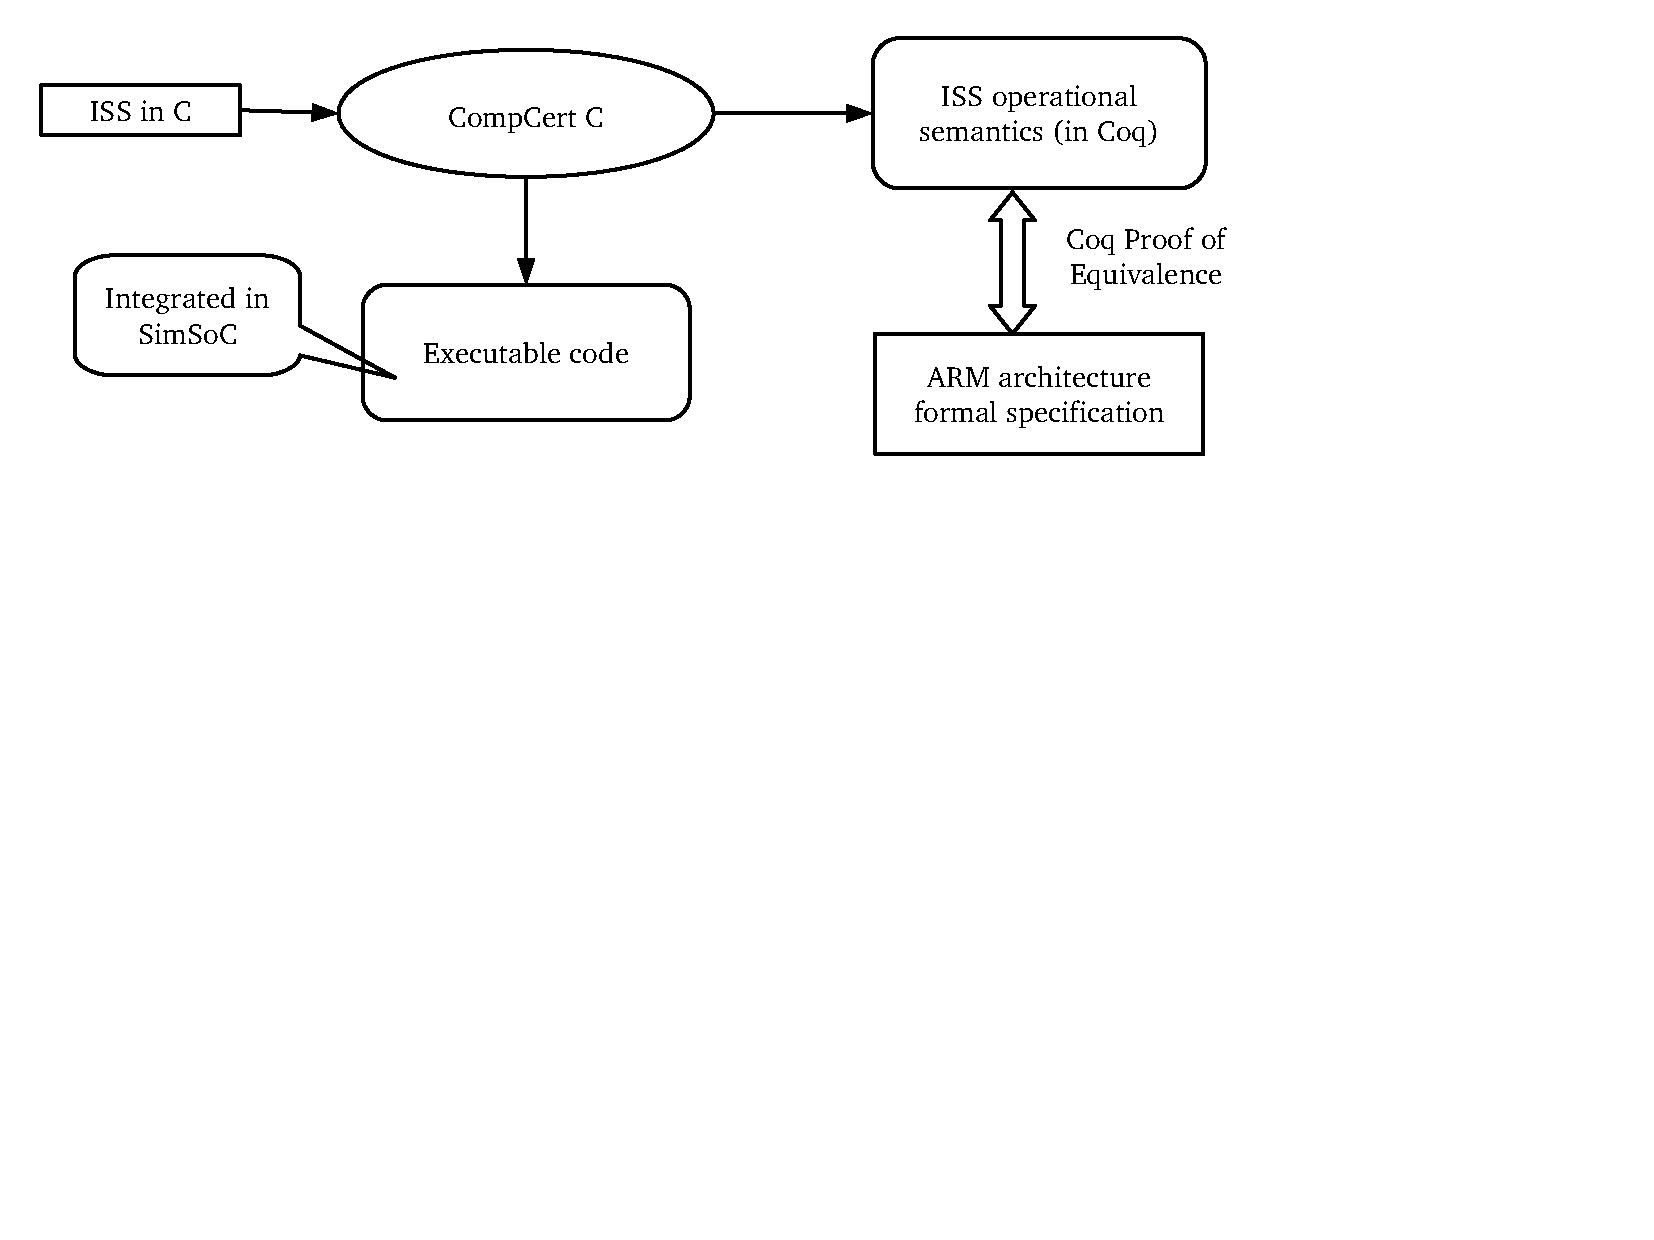
\includegraphics[width=0.9\linewidth, trim= 7mm 133mm 55mm 6mm, clip=true]
{newdiag.pdf}
\caption{Overall goal}
\label{fig:diagram}
\end{figure}

The general objective is to obtain a verified simulator is illustrated in
Figure~\ref{fig:diagram}.  Considering the ARM architecture, we need
to have the following:\begin{itemize}\itemsep=0pt
\item a formal model of the ARM instruction set.
\item an instruction set simulator of the ARM arcchitecture coded in
  the (\compcert) C programming language.
\item a formal operational semantics of the ISS. As shown in
  Figure~\ref{fig:diagram}, from the ISS source code in C, we can
  obtain through \compcert C on one hand
  the Coq formal semantics of the compiled C program constructed by
  \compcert, since the intermediate representation of the C compiler
  is a Coq representation
%  or alternatively
  and, on the other hand,
  the verified machine code,
  which conforms to this operational semantics as guaranteed by CompCert.
  We use both, the compiled machine code to
  run simulations, and the formal semantics for the proof.
\item prove, using the Coq proof assistant, that the resulting ISS semantics
  indeed implement the formal model of the ARM processor, which boils
  down to verifying that the semantics of the simulator accurately
  modifies the processor (and memory) state representation at each
  step and ends up in results that comply with the
  formal model of the ARM architecture.
\end{itemize}

These steps are described in the following paragraphs.


\subsection{Constructing the formal model}

Ideally the formal specification of the ARM architecture should be
provided by the vendor. But it is not the case,
an issue already raised
in the work with HOL4 mentioned above~\cite{FoxM10}.
% such a formal model is not available on their web site,
%% hence we had to build one
%% The only document available is
%% the ARM reference manual \cite{arm6refman}.
% (version 6 for this work).
We decided to derive
% So, it was elected to define
the formal
model of ARM architecture in Coq from the architecture
reference manual as output of a semi-automated process. The main
relevant chapters of the manual are:
\begin{itemize}
\item
\texttt{Programmer's Model} introduces the main features in ARMv6 architecture,
the data types, registers, exceptions, etc;
\item
\texttt{The ARM Instruction Set}
explains the instruction encoding in general and puts the instructions in
categories;
\item \texttt{ARM Instructions} lists all the ARM instructions in
  ARMv6 architecture in alphabetical order and the \texttt{ARM
    Addressing modes} section explains the five kinds of
  addressing modes.
\end{itemize}

There are 147 ARM instructions in the ARM V6 architecture.  For each
instruction, the manual provides its encoding table, its syntax, a
piece of pseudo-code explaining its own operation, its exceptions,
usage, and notes.
% %Need room...
%  Except the semi-formal pseudo-code, everything else
% is written in natural language.
%
Three kinds of information are extracted for each ARM operation: its
binary encoding format, the corresponding assembly syntax, and the
instruction semantics, which is an algorithm operating on
% the variousdata structures representing the state of an ARM processor, mostly
%registers and memory, according to the purpose of the instruction
the processor state. This algorithm may call basic functions defined
elsewhere in the manual, for which we provide a Coq library defining
their semantics. Other than these extracted data files, there is still
useful information left in the document which cannot be automatically
extracted, such as validity constraints information required by the
decoder generator.  However, the most tedious (then, arguably, error
prone) part is described using fairly simple, precise and regular
pseudo-code, allowing us to extract the Coq formal model in three
automated steps: (i) extracting information from the \texttt{.pdf}
file;
% %Need room...
% completed with some manual patch to express the relevant constraints
(ii) parsing the
data into abstract syntax trees
%with a parser generated from grammar;
(iii) automated translation from the abstract syntax into Coq formal
model.

During this process, a dozen documentation problems were found but
none that were relevant to instruction semantics. These documentation
mistakes have been acknowledged by ARM Ltd.  Moreover, a single
mistake in our automated extractor would impact the formal model of
many or even all instructions and then become rather easy to detect.
The model has then tested on real programs to verify that we obtain
the same results, which gives reasonable confidence in the model.

\subsection{Proof Structure}

The proof starts from an ISS coded in C, where each instruction is
coded as a C function that modifies the processor state and possibly
the memory state (but everything is represented in memory on the
simulation host machine). Each C function may also call basic
functions from a library. As mentioned above, this C code does not
include any construction with ``unspecified behavior'' of the C
language specification. To prove that the simulator is correct, we
need to prove that, given the initial state of the system, the
execution of an instruction as implemented by a C function results in
the same state as the formal specification. To establish the proof, a
formal model of that C implementation is provided by \compcert, which
defines operational semantics of C formalized in Coq.

\begin{figure}[htb]
\hfil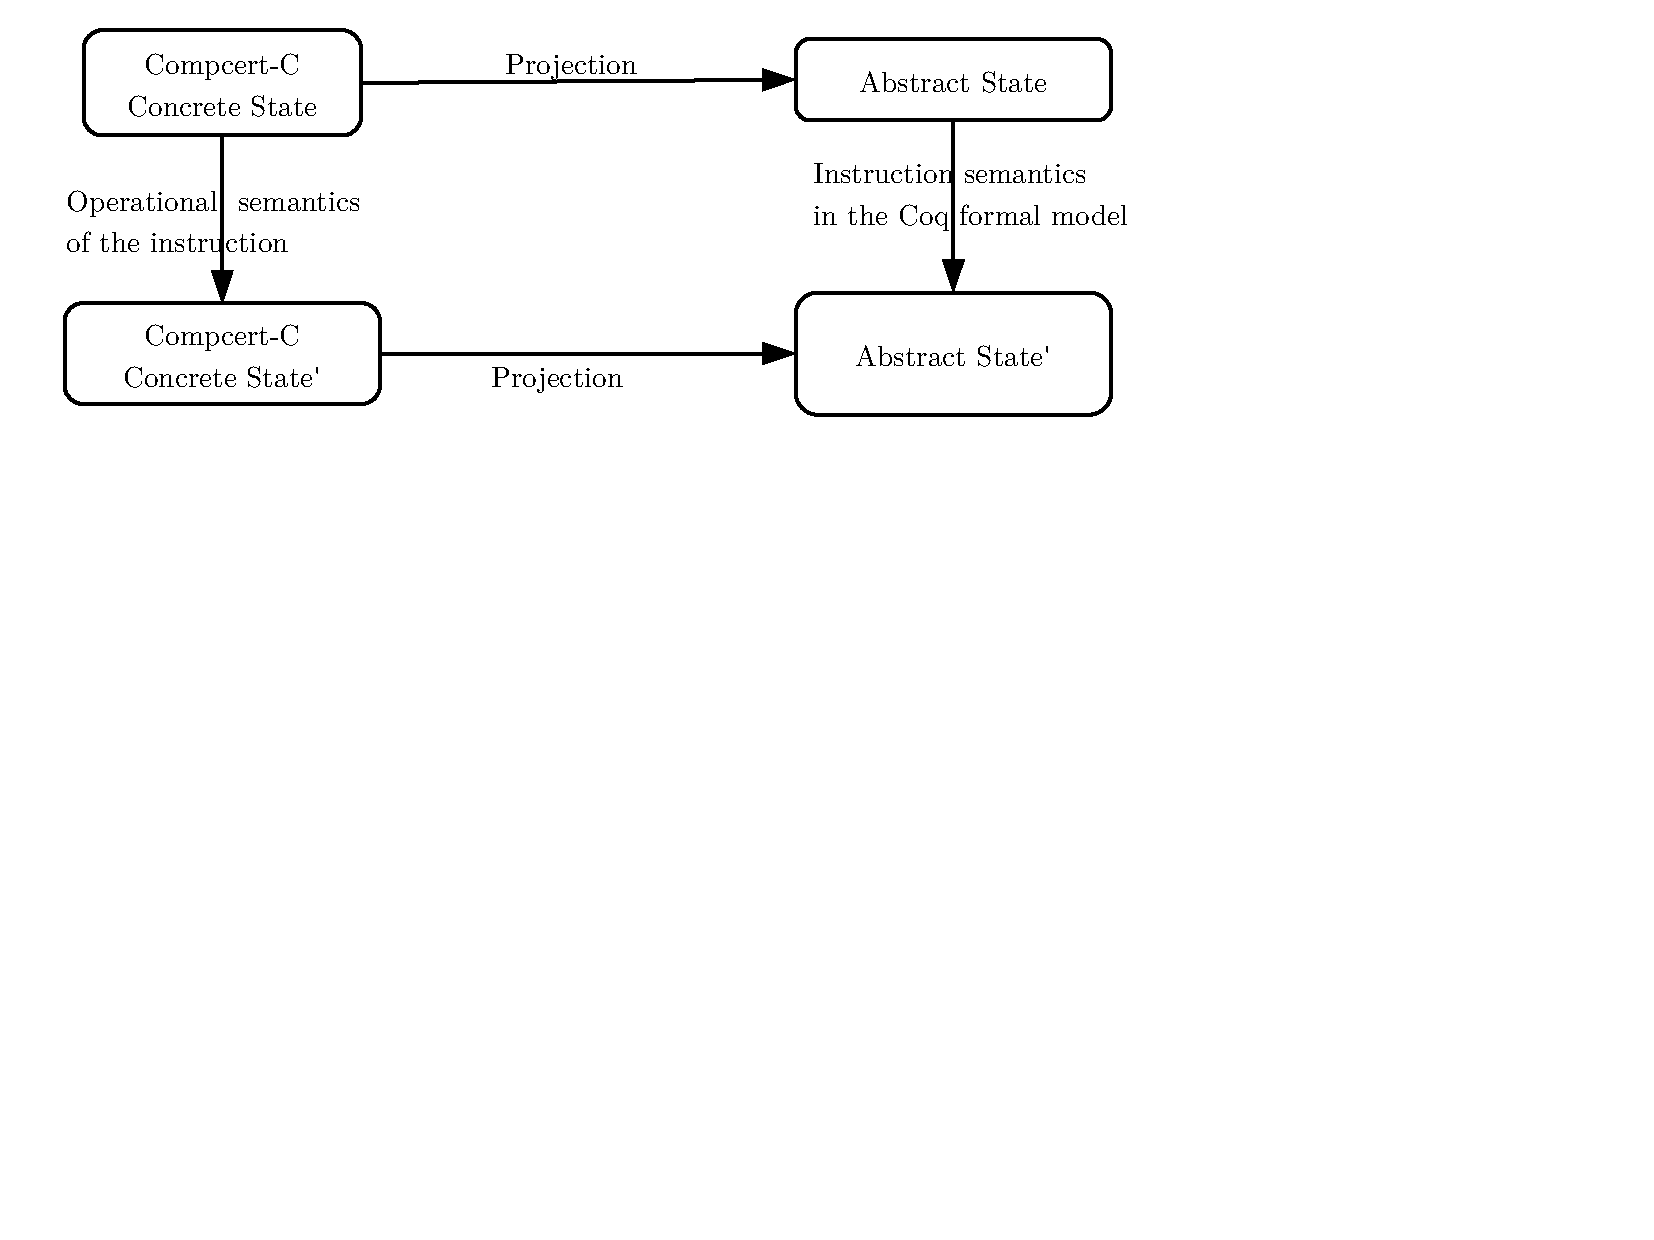
\includegraphics[width=0.9\linewidth, trim= 10mm 138mm 60mm 5mm, clip=true]{newproj.pdf}
\caption{Theorem statement for a given ARM instruction}
\label{fig:theoca}
\end{figure}

The proof shall demonstrate that the operational semantics of the C
code corresponds to the ARM formal specification. The complete proof
is too lengthy for this article, and we only provide here an outline
of the method.  The state of the ARM V6 processor defined in the
formal model is called the \emph{abstract state}.  Alternatively, the
same state is represented by the data structures corresponding to C
semantics that we shall call the \emph{concrete state}.  In order to
establish correctness theorems we need to relate these two models.
Executing the same instruction on the two sides produces a pair of new
processor states which should be related as equivalent. Informally,
executing the same instruction on a pair of equivalent states should
produce a new pair of equivalent states, as schematized by
Figure~\ref{fig:theoca}.
%
Equivalent states are defined according to a suitable projection
from the C concrete state to the abstract model, as represented in
Figure~\ref{fig:proj}. This projection constructs a formal structure
from the concrete one. The formal structure obtained should be identical
to that obtained through the formal model, otherwise the C code is incorrect.
\begin{figure}[h]
\hfil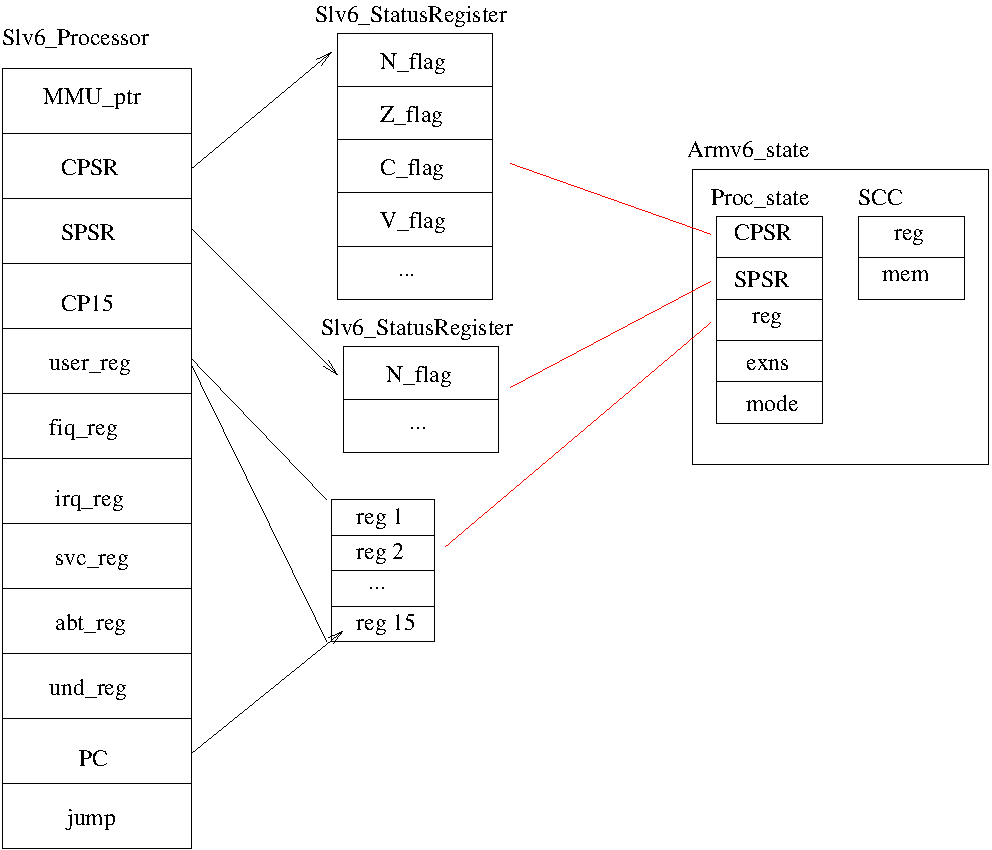
\includegraphics[width=.75\linewidth]{projection.pdf}
\caption{Projection}
\label{fig:proj}
\end{figure}

\subsection{Projection}
In order to achieve a high speed simulation, the C ISS includes
optimizations. In particular, processor state representation in the C
implementation is complex, not only due to the inherent complexity of
the C language memory model, but also because of optimization and
design decisions targeting efficiency.  Despite the complexity of the
C memory model, the \compcert C semantics makes it possible to define
and prove the projection. Fortunately, all of the
instructions operate on the processor state and there is a single
representation of that state in the simulator. It is necessary and
sufficient to prove the projection for each variant case of the
representation structure. For example, the projection of a register
performs a case analysis on possible values, whereas the projection of
saved data upon exceptions depends on the type of exception modes.
Although there are a number of specific cases to handle, the proof of
the projection is relatively straightforward.  In more detail:
\begin{itemize}
\item The C implementation uses large embedded \emph{struct}s to
  express the ARM processor state.  Consequently the model of the
  state is a complex Coq record type, including not only data fields
  but also proofs to verify access permission, next block pointer,
  etc.
\item Transitions are defined with a relational style (as opposed to a
  functional style where reasoning steps can be replaced by
  computations).
  % % JF: I feel the argument as somewhat dangerous, to be discussed.
  % % --> Xiaomu ?
  % As the kind of record type mentioned in the previous
  % item is too complex to execute computations with it, it is
  % convenient to describe the state transformations for memory with a
  % relation,
  % In simple situations functional style is lighter but its advantages
  % diminish in presence of dependent types.
  Relational style is more flexible,
  especially when dealing with constraints;
  and fits well with operational semantics.
\item The global state is based on a memory model with load
  and store functions that are used for read/write operations.
\end{itemize}

The proofs for instructions start from the abstract state described by
the formal specification.  To verify the projection of the
original state, we need the following data: the initial
memory state, the local environment, and the formal initial processor
state.  The projection is meaningful only after the C memory state is
prepared for evaluating the current function body representing a ARM
instruction.  In the abstract Coq model, we directly use the processor
state \texttt{st}.  But on the C side, the memory state is described
by the contents of several parameters, including the memory representation
of the processor state.  We also need to observe the modifications of
certain memory blocks corresponding to local variables.

% Fortunately \compcert formalizes the C memory model.
The semantics of \compcert C considers two environments. The global
environment \emph{genv} maps global function identifiers, global
variables identifiers to their blocks in memory, and function pointers
to a function definition body.  The local environment \emph{env} maps
local variables of a function to their memory blocks reference.  It
maps each variable identifier to its location and its type, and its
value is stored in the associated memory block.  The value associated
to a C variable or a parameter of a C function is obtained by applying
\texttt{load} to the suitable reference block in memory.  These two
operations are performed when a function is called, building a local
environment and an initialized memory state. When the program starts
its execution, \emph{genv} is built.  The local environment \emph{env}
is built when the associated function starts to allocate its
variables. Therefore, on the concrete side, a memory state and a local
environment is prepared initially using two steps. First, from an
empty local environment, all function parameters and local variables
are allocated, resulting into some memory state and the local
environment. Second, function parameters are set up using a dedicated
function \texttt{bind\_parameters} and the initial state is thus
created.

\subsection{Lemmas Library}

Next, we need to consider the execution of the instruction.
In the C ISS, there is a standalone C function
for each ARM V6 instruction.  Each function (instruction) has its own
correctness proof.  Each function is composed of its return
type, arguments variables, local variables, and the function body. The
function body is a sequence of statements including assignments and
expressions. Let us consider as an example the ARM instruction
\texttt{BL} (\texttt{Branch and Link}). The C code is:
%% JF HERE WE HAD A WRONG \small{ ==> scope until the end !!
{\small
\begin{verbatim}
void B(struct SLv6_Processor *proc,
       const bool L,
       const SLv6_Condition cond,
       const uint32_t signed_immed_24){
 if (ConditionPassed(&proc->cpsr, cond)){
  if ((L == 1))
   set_reg(proc,14,address_of_next_instruction(proc));
   set_pc_raw(proc,reg(proc,15)+(SignExtend_30(signed_immed_24)<<2));
 }
}
\end{verbatim}
}

\compcert has designed semantics for \compcert C in big-step inductive
types for evaluating expressions, which we reuse for the proof.  The
semantics is defined as a relation between an initial expression and
an output expression after evaluation.  Then, the body of the function
is executed.  On the concrete side, the execution yields a new state
\textbf{mfin}.  On the abstract side, the new state is
obtained by running the formal model.
% The formal model of ARM V6 is defined as a much simpler functional
% model and computing the value of a component can be performed
% directly.
We have to verify that the projection from the
concrete state \textbf{mfin} is related to this abstract
state.
% Note that all projections are
The proof is performed in a top-down manner. It follows the definition
of the instruction, analyzing the expression step by step.  The
function body is split into statements and then into expressions.
When evaluating an expression, one has to search for two kinds of
information. The first one is how the memory state changes on the
concrete side; the other is whether the results on the abstract and
the concrete model are related by the projection.  To this end, a
library of lemmas had to be developed, identifying five categories
summarized below.

%\begin{enumerate}
%\item
\medskip\noindent
  \textit{1. Evaluating a \compcert expression with no modification on the memory state.}\\
  Such lemmas are concerned with the expression evaluation on \compcert
  C side and in particular the C memory state change issue.  Asserting
  that a memory state is not modified has two aspects: one is that the
  memory contents are not modified; the other is that the memory
  access permission is not changed.  For example, evaluating the
  boolean expression $Sbit~==~1$ returns an unchanged memory state.
\[
\begin{array}{l}
\textrm{if}~~ G,E~\vdash \texttt{eval\_binop}_c~(Sbit~==~1),
\:M~\xLongrightarrow{\varepsilon}~v,\:M'
\\
\textrm{then}~~ M=M'.
\end{array}
\]
In Coq syntax, the relation in premise is expressed with
\texttt{eval\_binop}.
%a companion predicate of \texttt{exec\_stmt} above, devoted to binary operations.
In this lemma and the following,
$E$ is the local environment, $G$ is the global environment, $M$ is
the memory state, $\varepsilon$ is the empty event
% (\texttt{Events.E0} in Coq syntax);
(we may have here a series of events, e.g. system call, volatile
load/store) and $v$ is the result.
%(we may have here a series of events) and $v$ is the result.
% Here, $vres$ is not important.
The evaluation is performed under environments $G$ and $E$.  Before
evaluation, we are in memory state $M$.  With no event occurring, we
get the next memory state $M'$. According to the definition of
\texttt{eval\_binop}, an internal memory state will be introduced.
\begin{center}
$\dfrac
{G,E~\vdash a_1,M\Rightarrow M'~~~G,E~\vdash a_2,M'\Rightarrow M''
}
{G,E~\vdash (a_1~binop~a_2),M\Rightarrow~M''}$
\end{center}

In the example, expression $a_1$ is the value of $Sbit$ and $a_2$
is the constant value $1$.  By inverting the hypothesis of type
\texttt{eval\_binop}, we obtain several new hypotheses, including on
the evaluation of the two subexpressions and the introduction of an
intermediate memory state $M''$.  Evaluating them has no change on the
C memory state, hence we have $M = M'' = M'$.
In more detail, from the \compcert C semantics definition, we know that
the evaluation of an expression will change the memory state
if the evaluation contains uses of \texttt{store\_value\_of\_type}.
% in \compcert versions before 1.11.
% which stores the value in memory at a given block reference and
% memory chunk.
In \compcert, the basic store function on memory
is represented by an inductive type \texttt{assign\_loc} instead of
\texttt{store\_value\_of\_type}.
As a note, since \compcert version supports volatile memory access,
we also have to determine whether the object type is volatile before storage.
% and also type size in addition of the access mode.

%\item
\medskip\noindent
\textit{2. Result of the evaluation of an expression with no modification on the memory.}\\
Continuing the example above, we now discuss the result of evaluating
the binary operation $Sbit~==~1$ both in the abstract and the concrete model.
At the end of evaluation, a boolean value $true$ or $false$ is returned
in both the concrete and the abstract models.
\[
\begin{array}{l}
\textrm{if} ~ \texttt{Sbit\_related}~M~\texttt{Sbit},\\
\textrm{and} ~ G,E~\vdash \texttt{eval\_rvalue\_binop}_c~(Sbit~==~1),  M\Rightarrow~v,M'\\
\textrm{then} ~ v=(Sbit~==~1)_{coq}
\end{array}
\]
Intuitively, the projection corresponding to the parameter
\texttt{sbit} in the concrete model must yield the same value as in
the abstract model.  Here, the expression is a so-called ``simple
expression'' that always terminates in a deterministic way, and
preserves the memory state.  To evaluate the value of simple
expressions, \compcert provides two big-step relations
\texttt{eval\_simple\_rvalue} and \texttt{eval\_simple\_lvalue} for
evaluating respectively their left and right values.  The rules have
the following shape:
\[
\dfrac{
\begin{array}{l}
G,E~\vdash a_1,M\Rightarrow v_1 \quad G,E~\vdash a_2,M\Rightarrow v_2\\
\texttt{sem\_binary\_operation}(op,v_1,v_2,M)~=~v
\end{array}}
{G,E~\vdash (a_1~op~a_2),M\Rightarrow v}
\]
In order to evaluate the binary expression $a_1~op~a_2$,
the sub-expressions $a_1$ and $a_2$ are first evaluated,
and their respective results $v_1$ and $v_2$ are used
to compute the final result $v$.

%\item
\medskip\noindent
  \textit{3. Memory state changed by storage operation or side effects.}\\ % of evaluating expression
  As mentioned before, evaluating some expressions such as
  \texttt{eval\_assign} may modify the memory state.  Lemmas are
  required to state that corresponding variables in the abstract and
  in the concrete model must evolve consistently.  For example,
  considering an assignment on register $Rn$, the projection relation
  \texttt{register\_related} is used. Expressions with side effects of
  modifying memory are very similar.
\[
\begin{array}{l}
\textrm{if} ~~ \texttt{rn\_related}~M~rn\\
\textrm{and}~~  G,E~\vdash \texttt{eval\_assign}_c~(rn:=rx),M~\Rightarrow~ M',v\\
\textrm{then} ~~ \texttt{rn\_related}~M'~rn
\end{array}
\]

%\item
\medskip\noindent
  \textit{4. Internal function call.}\\
  The simulation code is sometimes using functions from libraries.
%  One needs to verify potential issues from these calls.
  We   distinguish \texttt{internal} functions and \texttt{external}
  functions.  An internal function is a function that belongs to a
  library, the code of which is part of the simulator, that we have
  coded ourselves, or the C code is provided by compcert C.  An
  external function is a function for which we do not have access to
  the operational semantics.  After an internal function is called, a
  new stack of blocks is typically allocated in memory.  After the
  evaluation of the function, these blocks will be freed.
  Unfortunately, this may not bring the memory back to the previous
  state: the memory contents may stay the same, but pointers and
  memory organization may have changed.
  \label{page:libfunast}
  \[
  \begin{array}{l}
    \textrm{if} ~~  \texttt{proc\_state\_related}~M~st \\
    \textrm{and} ~~ G,E~\vdash \texttt{eval\_funcall}_c (copy\_StatusRegister)_c,M\Rightarrow~v,~M'\\
    \textrm{and} ~~ st'~=~(copy\_StatusRegister)_{coq}~st\\
    \textrm{then} ~~\texttt{proc\_state\_related}~M'~st'.
  \end{array}
  \]

  Lemmas must be developed regarding the evaluation of internal
  functions, so that one can observe the returned results,
  compare it with the corresponding evaluation in the formal
  specification, and verify some conditions.  For example, the lemma
  above is about the processor state after evaluating an internal
  function call \texttt{copy\_StatusRegister}, which reads the value of
  the CPSR (Current Processor Status Register) and copies it into
  the SPSR (Saved Processor Status Register) when an exception occurs.  The
  evaluation of \texttt{copy\_StatusRegister} must be protected by a
  check on the current processor mode.  If it is in authorized mode, the
  function \texttt{copy\_StatusRegister} can be called.  Otherwise, the
  result is ``unpredictable'', which is defined by ARM architecture

  It is necessary to reason on the newly returned states, which
  should still be related by the projection.  This step is usually easy
  to prove, by calculation on the two representations of the processor
  state to verify that they match.

%\item
\medskip\noindent
  \textit{5. External function call.}\\
  The \compcert C AST of an external function call contains the types
  of input arguments and of the returned value, and an empty body.
  For each external function (e.g. \texttt{memcpy()}), we have its
  asserted properties. mostly provided by \compcert C.  The general
  expected properties of an external call are that (i) the call
  returns a result, which has to be related to the abstract state,
  (ii) the arguments must comply with the signature.  (iii) after the
  call, no memory blocks are invalidated, (iv) the call does not
  increase the access permission of any valid block, and finally that
  the memory state can be modified only when the access permission of
  the call is granted. For each external call, such required
  properties are verified.
%\end{enumerate}

%% JF Not crucial
% In addition to the above lemmas we had to prove a fair number of more
% trivial lemmas that are omitted here.  Most of them are related to the
% semantics of \compcert C. They are all gathered into a library of
% lemmas used to construct the individual instructions proofs.

\subsection{Inversion}
% Details are given in~\cite{xiaomu-phd}.
Equipped with these lemmas we can build the proof scripts for ARM
instructions.  For that, we are decomposing the ARM instruction
execution step by step to perform the execution of the C programs.
\compcert C operational semantics define large and complex inductive
relations. Each constructor describes the memory state transformation
of an expression, statement, or function.  As soon as we want to
discover the relation between memory states before and after
evaluating the C code, we have to \emph{invert} the hypotheses of operational
semantics to follow the clue given by its definition, to verify the
hypotheses relating concrete memory states according to the
operational semantics.

% During the development of a proof, if a hypothesis is an instance of
% an inductive predicate and we want to derive the consequences of this
% hypothesis, the general logical principle to be used is called
% \emph{inversion}.
An \emph{inversion} is a kind of forward reasoning
step that allows for users to extract all useful information contained
in a hypothesis.  It is an analysis over the given hypothesis according
to its specific arguments, that removes absurd cases, introduces
relevant premises in the environment and performs suitable
substitutions in the whole goal.
% The practical need for automating
%inversion has been identified many years ago and
Most proof assistants provide an inversion mechanism.
In the case of Coq, it is
a general tactic called
\inversion~\cite{coqmanual}.

Every instruction contains complex expressions, but each use of
\inversion will go one step only.  If we want to find the relation
between the memory states affected by these expressions, we have to
invert many times. For illustration, let us consider the simple
example from the ARM reference manual \texttt{CPSR = SPSR}, that
assigns to register CPSR the value of SPSR (defined above).  As the
status register is not implemented by a single value, but a set of
individual fields, the corresponding C code is a call to the function
\texttt{copy\_StatusRegister}, which sets the CPSR field by field with
the values from SPSR.  Lemma \texttt{same\_cp\_SR} below states that
the C memory state of the simulator and the corresponding formal
representation of ARM processor state evolve consistently during this
assignment.
\begin{alltt}\small
Lemma same_copy_SR :
  \(\forall\) e m l b s t m' v em,
  proc_state_related m e (Ok tt (mk_semstate l b s)) \(\rightarrow\)
    eval_expression (Genv.globalenv prog_adc) e m expr_cp_SR t m' v  \(\rightarrow\)
    \(\forall\) l b, proc_state_related m' e
                      (Ok tt (mk_semstate l b (Arm6_State.set_cpsr s
                                              (Arm6_State.spsr s em))))
\end{alltt}
In its proof, 18 consecutive inversions are needed in order to exhaust
all constructors occuring in the assumptions.  Unfortunately,
\inversion generates uncontrolable names which pollute proof scripts.
Here, an intensive use of \inversion makes proofs scripts
unmanageable, and not robust to version changes of Coq or \compcert.
%
In order to reduce the script size and get better
maintainability, we studied a general solution to the inversion problem,
and developed a new mechanism described in~\cite{itp13}.
%\cite{small-inversion,itp13}
% The standard inversion mechanism from Coq has been expanded into a new
% inversion tactic for inductive types in \compcert.  The semantics of
% \compcert C tells how the memory state is transformed by evaluating
% expressions.  Using the built-in constructs of the tactics language,
% one can define a high-level tactic for each inductive type, gathering
% all the functions defined for its constructors.
%
On top of it, we could program a Coq tactic able to
% The new tactic
automatically find the hypothesis to invert by matching the targeted
memory states,
properly manage other hypotheses,
perform our inversion,
clean up the goal,
and repeat
% then to revert related hypotheses,
% Next, all other related hypotheses are updated according to the new names,
% and finally new values and useless variables or hypotheses are cleaned up.
the above steps until all transitions between the
two targeted memory states are discovered.

As a result, proofs script have become much shorter and more manageable.
Considering the former example of \texttt{same\_copy\_SR},
the 18 calls to standard \inversion
reduce into one single step:
\texttt{inv\_eval\_expr~m~m'}.

\subsection{Instruction Proofs}
Proofs of instructions rely heavily on
the library of lemmas and the controlable inversion mechanism
described above.
Scripts size vary with the instructions complexity from less than 200 lines (e.g
170 for LDRB) to over 1000 (1204 for ADC).
As a result, for each ARM instruction,
we have established a theorem proving that the C code
simulating an ARM instruction is equivalent to the formal
specification of the ARM processor.

% \section{Certified Simulation}

% Based on the work afore mentioned, we can now consider the certified
% execution of a C program. We take here as an example the DES
% cryptographic encryption code.  The C code for encrypting a block of
% data is straightforward:
%
% {\small\begin{verbatim}
% #define GET_ULONG_BE(n,b,i)
%  (n)=((unsigned long)(b)[(i)]<<24)
%     |((unsigned long)(b)[(i)+1]<<16)
%     |((unsigned long)(b)[(i)+2]<<8)
%     |((unsigned long)(b)[(i)+3] );

% #define DES_IP(X,Y)
%     T =((X>>4)^Y)&0x0F0F0F0F;
%     Y^=T;X^=(T<<4);
%     T=((X>>16)^Y)&0x0000FFFF;
%     Y^=T;X^=(T<<16);
%     T=((Y>>2)^X)&0x33333333;
%     X^=T;Y^=(T<<2);
%     T=((Y>>8)^X)&0x00FF00FF;
%     X^=T;Y^=(T<<8);
%     Y=((Y<<1)|(Y>>31))&0xFFFFFFFF;
%     T=(X^Y)&0xAAAAAAAA;
%     Y ^=T;X^= T;
%    X=((X<<1)|(X>>31))&0xFFFFFFFF;

% #define DES_ROUND(X,Y)
%     T=*key++^X;
%     Y^=SB8[(T)&0x3F]
%        ^SB6[(T>>8)&0x3F]
%        ^SB4[(T>>16)&0x3F]
%        ^SB2[(T>>24)&0x3F];
%     T=*key++^((X<<28)|(X>>4));
%     Y^=SB7[(T)&0x3F]
%        ^SB5[(T>>8)&0x3F]
%        ^SB3[(T>>16)&0x3F]
%        ^SB1[(T>>24)&0x3F];

% void des_crypt_ecb(unsigned long *key,
%                unsigned char input[8],
%              unsigned char output[8] ){
%     int i;
%     unsigned long X,Y,T;
%     GET_ULONG_BE(X,input,0);
%     GET_ULONG_BE(Y,input,4);
%     DES_IP(X,Y);
%     for(i=0;i<8;i++) {
%         DES_ROUND(Y,X);
%         DES_ROUND(X,Y);
%     }
%     DES_FP(Y,X);
%     PUT_ULONG_BE(Y,output,0);
%     PUT_ULONG_BE(X,output,4);
% }
% \end{verbatim}
% }

% Looking at the binary code of that function generated by the compiler,
% one may observe that this code actually uses only 22 different types of ARM
% instructions, namely \textbf{ add, and, asr, b, ble, bne, bx, cmp,
%   eor, ldm, ldr, ldrb, lsl, lsr, mov, orr, pop, push, str, str, strb,
%   sub}.

% Given that we have a proof that the machine code generated from C is
% correct, thanks to \compcert, and now a proof of the ARM instruction
% set for these instructions, we have a proof that the simulation of the
% DES algorithm on our ARM simulator is conformant with the algorithm.


%%%%%%%%%%%%%%%%%%%%%%%%%%%%%%%%%%%%%%%%%%%%%%%%%%%%%%%%%%%%%%%%%
\section{Conclusion}
\label{conclusion}

Using the approach presented in this paper, we have constructed a tool
chain that makes it possible to certify that the simulation of a
binary executable program on some simulation platform is compliant
with the formal model of the target hardware architecture.
Using Compcert-C, that has defined formal C semantics, we have
formally proved, using the Coq theorem prover,
the ARM v6 Instruction Set Simulator of SimSoc.
%  There is no limit on
%the size of the code that can be simulated as long as the target
% instruction set has been certified.

We certainly acknowledge the limits of our approach: the quality of
our ``verified simulation'' relies on the faithfulness of our formal
model of the ARM processor to the real hardware. Because the vendor
companies do not provide a formal description of their hardware, one
has to build them\footnote{Note that this problem is the same as for
  the work done by Cambridge University.}.
This issue is partly solved in this work
by automatically deriving
the most tedious parts of the Coq formal model
from pseudo-code extracted from the vendor reference manual.
% by extracting the pseudo-code from the manual and
% translating this code into a Coq formal model.
% Another potential issue
%is that ARM is licensing the technology to electronics companies, and
%it is not certain either that the chips manufactured by these
%licensees are truly compliant with the original specification that
%they license, but this is well beyond the scope of this paper.
If the vendors would make public formal specifications of their
architectures, then our toolchain would become fully verified.

We believe this work has further impact on proofs of programs.  First,
we have proved here a significantly large C program.  Second, because
the proved program is a hardware simulator, it can be used as a tool
to prove execution of target programs.  For example considering a
cryptographic algorithm implemented for the ARM archiecture and
compiled with Compcert-C, it could then be proved that the execution
of that program provides the exact encryption required, and nothing
else.  Therefore, the tool presented is an enabler for the proofs of
other programs, which offers a direction for future research.

Another consequence of this work is that, supposing one could
compile the C instructions to silicon using a silicon compiler,
and that compiler would also be certified, ala \compcert,
it would then make it possible to prove real hardware...

% As a side note, the generator from the documentation also generates
% the decoder of binary instructions supported in ARM
% architectures. This decoder is obtained by compiling the opcodes
% information, so we are confident that the decoder from binary to call
% the appropriate C function is correct, and has been tested on
% hundreds of millions of cases.

%%%%%%%%%%%%%%%%%%%%%%%%%%%%%%%%%%%%%%%%%%%%%%%%%%%%%%%%%%%%%%%%%%
% \section*{Acknowledgments}

% Removed for review.
% This work has been supported jointly by INRIA, Tsinghua University
% and CNRS, Vania Joloboff is currently visiting Professor at East
% China Normal University.

%%%%%%%%%%%%%%%%%%%%%%%%%%%%%%%%%%%%%%%%%%%%%%%%%%%%%%%%%%%%%%%%%%


%\bibliographystyle{IEEEtran}
\bibliographystyle{abbrv}
\bibliography{references}


\end{document}
